\chapter{Perancangan}
\label{chap:perancangan}

\section{Perancangan Struktur Modul}
\label{sec:perancangan_struktur_modul}
Berdasarkan \textit{work-flow map} yang telah dirancang pada bab sebelumnya, maka dirancang struktur modul yang menjelaskan mengenai modul-modul apa saja yang akan dirancang untuk membangun \textit{website} SIKSA. Garis besar dari struktur modul ini terbagi menjadi 3 bagian berdasarkan penggunanya, yaitu modul mahasiswa, modul TU dan modul pejabat.\
Gambar \hyperlink{struktur_modul_garis_besar}{4.1} menjelaskan struktur modul secara garis besar.

\begin{figure}[H]
	\centering
		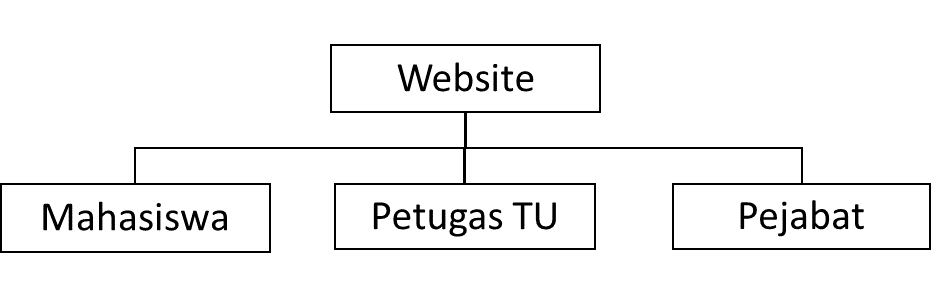
\includegraphics[scale=0.65]{F:/Skripsi/Dokumentasi_Skripsi/Gambar/Struktur_Modul/modul_utama.png}
	\caption{Struktur modul secara garis besar}
	\label{fig:struktur_modul_garis_besar}
\end{figure}

Selanjutnya, modul-modul yang telah disebutkan sebelumnya memiliki struktur tersendiri yang lebih spesifik. Gambar \hyperlink{struktur_modul_mahasiswa}{4.2} menjelaskan struktur modul mahasiswa secara menyeluruh.

\begin{figure}[H]
	\centering
		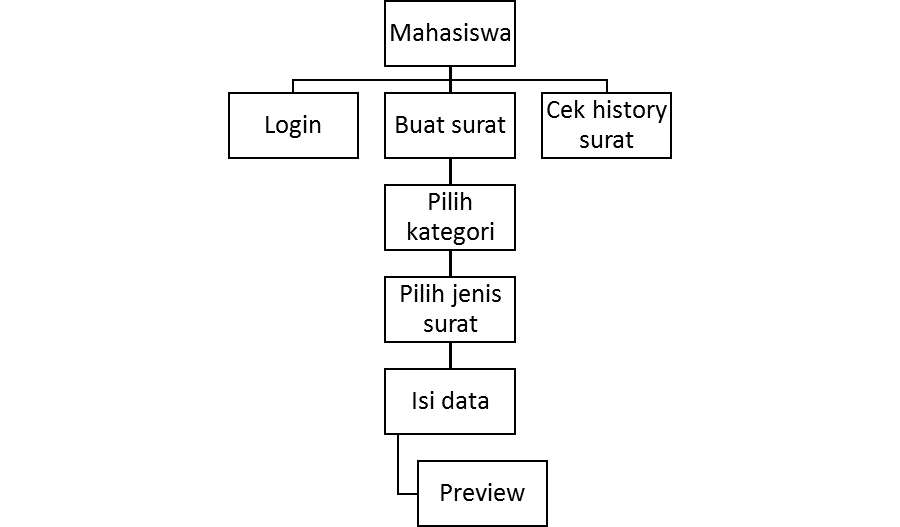
\includegraphics[scale=0.85]{F:/Skripsi/Dokumentasi_Skripsi/Gambar/Struktur_Modul/modul_mahasiswa.png}
	\caption{Struktur modul mahasiswa}
	\label{fig:struktur_modul_mahasiswa}
\end{figure}

Berdasarkan gambar di atas, berikut ini adalah penjelasan mengenai struktur modul mahasiswa dari \textit{website} SIKSA :
\begin{enumerate}
	\item Modul \textit{login}.
	\item Modul untuk membuat surat.
	\item Modul untuk mengecek \textit{history} pembuatan surat.
\end{enumerate}

Gambar \hyperlink{struktur_modul_tu}{4.3} menjelaskan struktur modul petugas TU secara menyeluruh.

\begin{figure}[H]
	\centering
		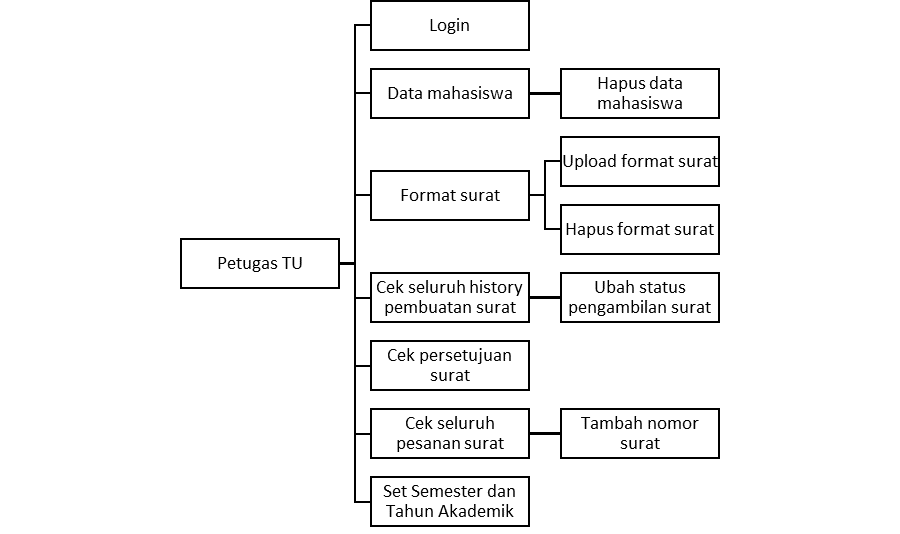
\includegraphics[scale=0.95]{F:/Skripsi/Dokumentasi_Skripsi/Gambar/Struktur_Modul/modul_TU-rev.png}
	\caption{Struktur modul petugas TU}
	\label{fig:struktur_modul_TU}
\end{figure}

Berdasarkan gambar di atas, berikut ini adalah penjelasan mengenai struktur modul TU dari \textit{website} SIKSA :
\begin{enumerate}
	\item Modul \textit{login}.
	\item Modul untuk melihat data mahasiswa.
	\item Modul untuk melihat format surat.
	\item Modul untuk mengecek seluruh \textit{history} pembuatan surat.
	\item Modul untuk mengecek seluruh pesanan surat yang masuk.
	\item Modul untuk mengubah semester dan tahun akademik terkini.
\end{enumerate}

Gambar \hyperlink{struktur_modul_pejabat}{4.4} menjelaskan struktur modul pejabat secara menyeluruh.

\begin{figure}[H]
	\centering
		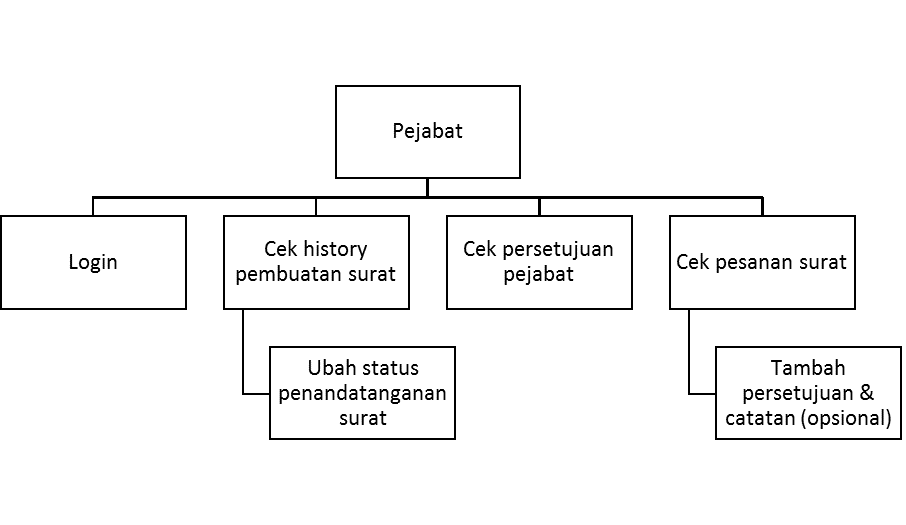
\includegraphics[scale=0.75]{F:/Skripsi/Dokumentasi_Skripsi/Gambar/Struktur_Modul/modul_pejabat.png}
	\caption{Struktur modul pejabat}
	\label{fig:struktur_modul_pejabat}
\end{figure}

Berdasarkan gambar di atas, berikut ini adalah penjelasan mengenai struktur modul pejabat dari \textit{website} SIKSA :
\begin{enumerate}
	\item Modul \textit{login}.
	\item Modul untuk mengecek \textit{history} pembuatan surat.
	\item Modul untuk mengecek pesanan surat yang masuk.
\end{enumerate}

\section{Perancangan Fisik Basis Data}
\label{sec:perancangan_fisik_basis_data}
Berdasarkan diagram ER yang telah dibuat pada bab III, dapat dibangun perancangan fisik dari basis data untuk mengimplementasikan hubungan antar entitas.\

Tabel 4.1-4.9 berikut ini menjelaskan entitas apa saja yang dibangun beserta dengan atribut-atribut pada entitas tersebut.

\begin{table}[H]
\centering
\caption{Tabel entitas mahasiswa}
\label{entitas_mahasiswa}
\begin{tabular}{|l|l|l|l|l|l|}
\hline
\textbf{Nama Field}&\textbf{Tipe Data}&\textbf{Panjang}&\textbf{Ket.}&\textbf{Null?}&\textbf{FK ke Relasi Lain}\\ \hline
Id&int&10&PK&Not null&\\ \hline
NIRM&varchar&255&&Not null&\\ \hline
NPM&varchar&255&&Not null&\\ \hline
Nama&varchar&255&&Not null&\\ \hline
Jurusan&int&11&FK&Not null&Jurusan\\ \hline
Fakultas&int&11&FK&Not null&Fakultas\\ \hline
Angkatan&int&11&&Not null&\\ \hline
Kota lahir&varchar&255&&Not null&\\ \hline
Tanggal lahir&date&&&Not null&\\ \hline
Foto&varchar&255&&Not null&\\ \hline
Dosen wali&int&11&FK&Not null&Dosen\\ \hline
Username&varchar&255&&Not null&\\ \hline
Kewarganegaraan&varchar&255&&Not null&\\ \hline
Semester&varchar&6&&Not null&\\ \hline
Tahun Akademik&varchar&9&&Not null&\\ \hline
\end{tabular}
\end{table}

\begin{table}[H]
\centering
\caption{Tabel entitas dosen}
\label{entitas_dosen}
\begin{tabular}{|l|l|l|l|l|l|}
\hline
\textbf{Nama Field}&\textbf{Tipe Data}&\textbf{Panjang}&\textbf{Ket.}&\textbf{Null?}&\textbf{FK ke Relasi Lain}\\ \hline
Id&int&10&PK&Not null&\\ \hline
NIK&varchar&255&&Not null&\\ \hline
Nama&varchar&255&&Not null&\\ \hline
Jurusan&int&11&FK&Not null&Jurusan\\ \hline
Fakultas&int&11&FK&Not null&Fakultas\\ \hline
Foto&varchar&255&&Not null&\\ \hline
Username&varchar&255&&Not null&\\ \hline
\end{tabular}
\end{table}

\begin{table}[H]
\centering
\caption{Tabel entitas jurusan}
\label{entitas_jurusan}
\begin{tabular}{|l|l|l|l|l|l|}
\hline
\textbf{Nama Field}&\textbf{Tipe Data}&\textbf{Panjang}&\textbf{Ket.}&\textbf{Null?}&\textbf{FK ke Relasi Lain}\\ \hline
Id&int&10&PK&Not null&\\ \hline
Kode jurusan&varchar&255&&Not null&\\ \hline
Nama&varchar&255&&Not null&\\ \hline
Ketua jurusan&int&11&FK&Not null&Dosen\\ \hline
\end{tabular}
\end{table}

\begin{table}[H]
\centering
\caption{Tabel entitas fakultas}
\label{entitas_fakultas}
\begin{tabular}{|l|l|l|l|l|l|}
\hline
\textbf{Nama Field}&\textbf{Tipe Data}&\textbf{Panjang}&\textbf{Ket.}&\textbf{Null?}&\textbf{FK ke Relasi Lain}\\ \hline
Id&int&10&PK&Not null&\\ \hline
Kode fakultas&varchar&255&&Not null&\\ \hline
Nama&varchar&255&&Not null&\\ \hline
Dekan&int&11&PK&Not null&Dosen\\ \hline
Wakil Dekan I&int&11&FK&Not null&Dosen\\ \hline
Wakil Dekan II&int&11&FK&Not null&Dosen\\ \hline
Wakil Dekan III&int&11&FK&Not null&Dosen\\ \hline\end{tabular}
\end{table}

\begin{table}[H]
\centering
\caption{Tabel entitas format surat}
\label{entitas_format_surat}
\begin{tabular}{|l|l|l|l|l|l|}
\hline
\textbf{Nama Field}&\textbf{Tipe Data}&\textbf{Panjang}&\textbf{Ket.}&\textbf{Null?}&\textbf{FK ke Relasi Lain}\\ \hline
Id&int&10&PK&Not null&\\ \hline
Id format&varchar&255&&Not null&\\ \hline
Jenis surat&varchar&255&&Not null&\\ \hline
Keterangan&varchar&255&&Not null&\\ \hline
Link format&varchar&255&&Not null&\\ \hline
\end{tabular}
\end{table}

\begin{table}[H]
\centering
\caption{Tabel entitas pesanan surat}
\label{entitas_pesanan_surat}
\begin{tabular}{|l|l|l|l|l|l|}
\hline
\textbf{Nama Field}&\textbf{Tipe Data}&\textbf{Panjang}&\textbf{Ket.}&\textbf{Null?}&\textbf{FK ke Relasi Lain}\\ \hline
Id&int&10&PK&Not null&\\ \hline
Tanggal buat&timestamp&&&Not null&\\ \hline
Pemohon&int&11&FK&Not null&Mahasiswa\\ \hline
Jenis surat&int&11&FK&Not null&Format surat\\ \hline
Data surat&text&65,535&&Not null&\\ \hline
Penerima surat&varchar&255&&Not null&\\ \hline
Persetujuan dosen wali&tinyint&1&&Not null&\\ \hline
Tanggal dosen wali&varchar&50&&Not null&\\ \hline
Persetujuan Kaprodi&tinyint&1&&Not null&\\ \hline
Tanggal Kaprodi&varchar&50&&Not null&\\ \hline
Persetujuan WD II&tinyint&1&&Not null&\\ \hline
Tanggal WD II&varchar&50&&Not null&\\ \hline
Persetujuan WD I&tinyint&1&&Not null&\\ \hline
Tanggal WD I&varchar&50&&Not null&\\ \hline
Persetujuan dekan&tinyint&1&&Not null&\\ \hline
Tanggal dekan&varchar&50&&Not null&\\ \hline
Count&int&11&&Not null&\\ \hline
\end{tabular}
\end{table}

\begin{table}[H]
\centering
\caption{Tabel entitas \textit{history} surat}
\label{entitas_history_surat}
\begin{tabular}{|l|l|l|l|l|l|}
\hline
\textbf{Nama Field}&\textbf{Tipe Data}&\textbf{Panjang}&\textbf{Ket.}&\textbf{Null?}&\textbf{FK ke Relasi Lain}\\ \hline
Id&int&10&PK&Not null&\\ \hline
Tanggal buat&timestamp&&&Not null&\\ \hline
Nomor surat&varchar&255&&Not null&\\ \hline
Perihal&varchar&255&&Not null&\\ \hline
Penerima surat&varchar&255&&Not null&\\ \hline
Pemohon&int&11&FK&Not null&Mahasiswa\\ \hline
Jenis surat&int&11&FK&Not null&Format surat\\ \hline
Link arsip&varchar&255&&Not null&\\ \hline
Penandatanganan&tinyint&1&&Not null&\\ \hline
Pengambilan&tinyint&1&&Not null&\\ \hline
Id pesanan surat&int&11&FK&Not null&Pesanan surat\\ \hline
\end{tabular}
\end{table}

\begin{table}[h]
\centering
\caption{Tabel entitas petugas TU}
\label{entitas_petugas_TU}
\begin{tabular}{|l|l|l|l|l|l|}
\hline
\textbf{Nama Field}&\textbf{Tipe Data}&\textbf{Panjang}&\textbf{Ket.}&\textbf{Null?}&\textbf{FK ke Relasi Lain}\\ \hline
Id&int&10&PK&Not null&\\ \hline
NIK&varchar&255&&Not null&\\ \hline
Nama&varchar&255&&Not null&\\ \hline
\end{tabular}
\end{table}

\section{Perancangan Antar Muka}
\label{sec:perancangan_antar_muka}
Berdasarkan struktur modul yang telah dijelaskan pada bagian sebelumnya, maka dirancang antar muka untuk memberikan tampilan pada setiap fitur yang terdapat pada \textit{website} SIKSA. Pada bagian sebelumnya telah disebutkan bahwa terdapat 3 aktor yang menjadi \textit{user} dari \textit{website} SIKSA ini. Ketiga \textit{user} tersebut yaitu mahasiswa, pejabat dan petugas TU. Masing-masing \textit{user} memilik antar muka yang berbeda-beda sesuai dengan fitur yang dapat dijalankannya.

Untuk dapat mengakses \textit{website} SIKSA ini setiap pengguna perlu melakukan \textit{login} dengan menggunakan \textit{username} dan \textit{password} yang dimiliki pada halaman \textit{login}. Gambar \hyperlink{halaman_login}{4.5} menunjukkan halaman login.
\begin{figure}[H]
	\centering
		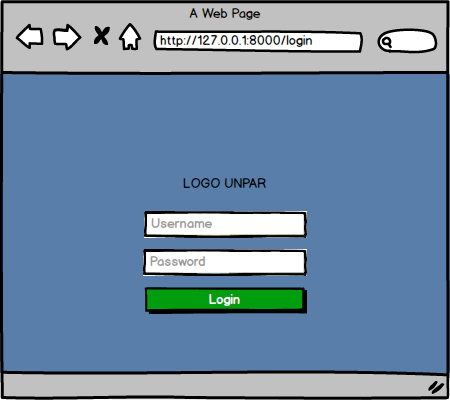
\includegraphics[scale=0.4]{F:/Skripsi/Dokumentasi_Skripsi/Gambar/Mock_Up/Login.png}
		\caption{Halaman \textit{login}}
		\label{fig:halaman_login}
	\end{figure}

\subsection{Perancangan Antar Muka Untuk Mahasiswa}
\label{sec:perancangan_antar_muka_mahasiswa}
Berdasarkan struktur modul, mahasiswa dapat menjalankan 2 fungsi yaitu membuat surat dan melihat surat yang sudah pernah dibuat yang akan dijelaskan sebagai berikut :

\begin{enumerate}
	\item Melihat surat yang sudah pernah dibuat\\
	Halaman \textit{home mahasiswa} adalah halaman yang ditampilkan apabila mahasiswa berhasil melakukan \textit{login}. Surat-surat yang pernah dibuat oleh mahasiswa ybs. akan ditampilkan pada halaman ini. Gambar \hyperlink{home_mahasiswa_yang_pernah_membuat_surat}{4.6} menunjukkan halaman \textit{home mahasiswa} yang menampilkan surat yang sudah pernah dibuat.

	\begin{figure}[H]
	\centering
		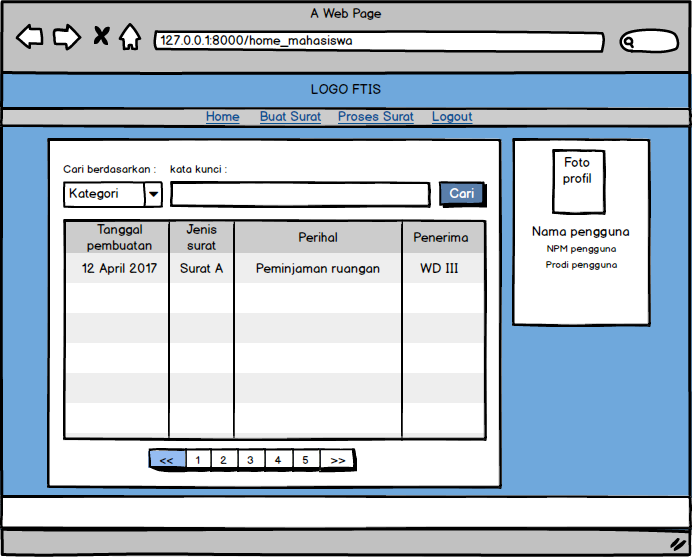
\includegraphics[scale=0.4]{F:/Skripsi/Dokumentasi_Skripsi/Gambar/Mock_Up/Mahasiswa/home_mahasiswa.png}
		\caption{Home mahasiswa yang pernah membuat surat}
		\label{fig:home_mahasiswa_yang_pernah_membuat_surat}
	\end{figure}
	
	Apabila mahasiswa ybs. belum pernah membuat surat sekalipun, maka tampilan untuk halaman \textit{home mahasiswa} akan menampilkan seperti pada gambar \hyperlink{home_mahasiswa_yang_belum_pernah_membuat_surat}{4.7} berikut.
	\begin{figure}[H]
	\centering
		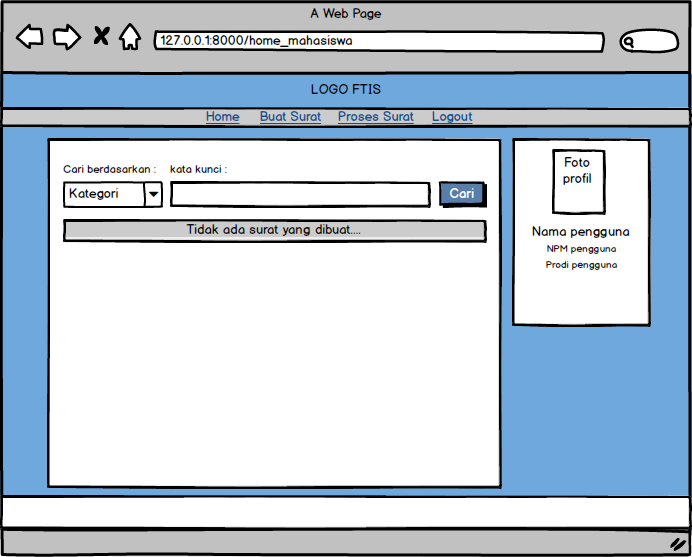
\includegraphics[scale=0.4]{F:/Skripsi/Dokumentasi_Skripsi/Gambar/Mock_Up/Mahasiswa/home_mahasiswa_kosong.png}
		\caption{Home mahasiswa yang belum pernah membuat surat}
		\label{fig:home_mahasiswa_yang_belum_pernah_membuat_surat}
	\end{figure}
	
	\item Membuat surat\\
	Untuk membuat surat mahasiswa perlu menekan menu "Buat Surat" pada \textit{navigation bar} untuk masuk ke halaman pemilihan kategori surat yang akan dibuat. Gambar \hyperlink{pilih_kategori_surat}{4.8} menunjukkan halaman pilih kategori surat.
	\begin{figure}[H]
	\centering
		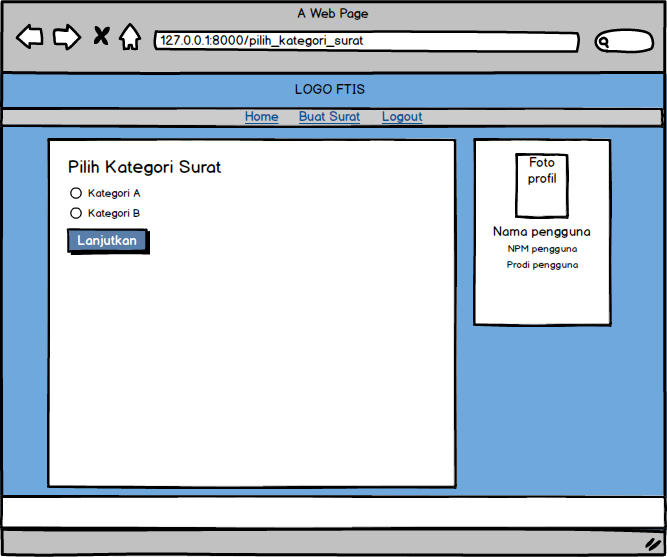
\includegraphics[scale=0.4]{F:/Skripsi/Dokumentasi_Skripsi/Gambar/Mock_Up/Mahasiswa/pilih_kategori_surat.png}
		\caption{Pilih kategori surat}
		\label{fig:pilih_kategori_surat}
	\end{figure}
	
	Setelah memilih kategori surat mahasiswa akan diarahkan ke halaman selanjutnya untuk memilih jenis surat yang akan dibuat. Gambar \hyperlink{pilih_jenis_surat}{4.9} menunjukkan halaman pilih jenis surat.
	\begin{figure}[H]
	\centering
		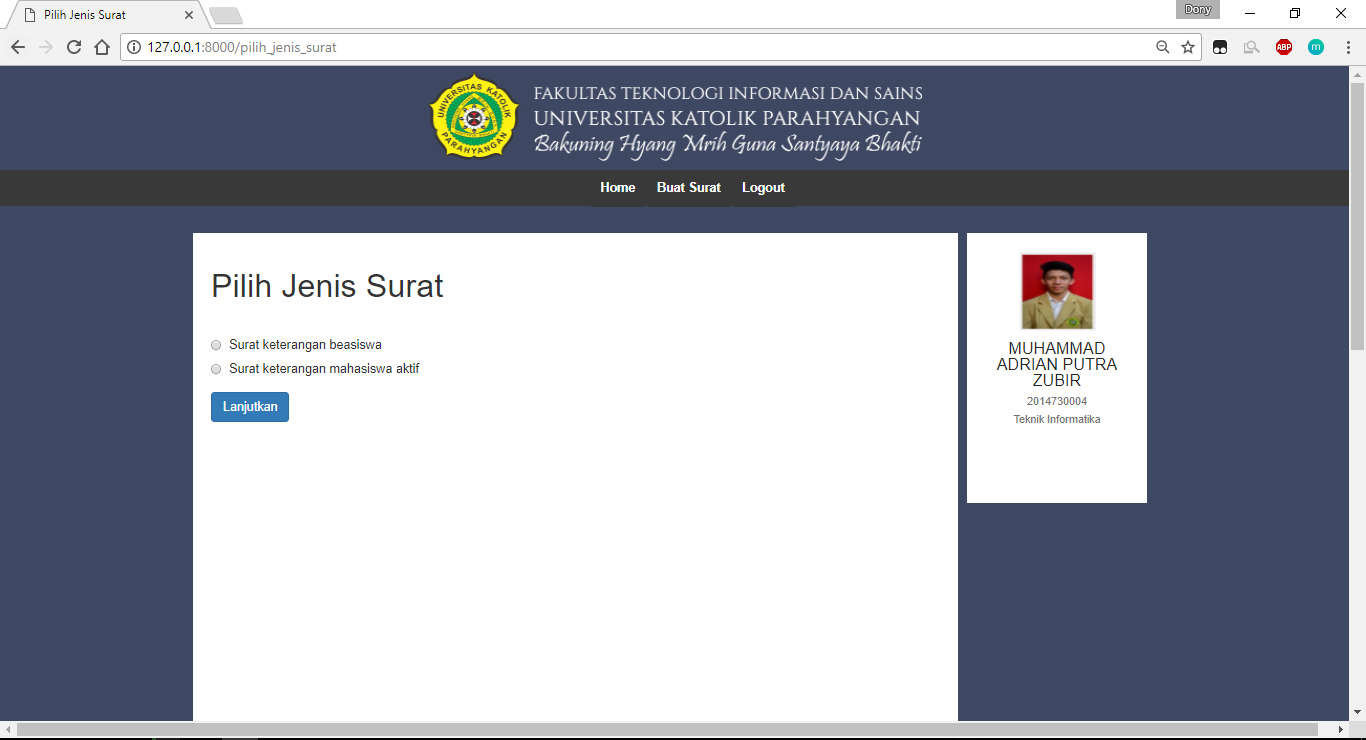
\includegraphics[scale=0.4]{F:/Skripsi/Dokumentasi_Skripsi/Gambar/Mock_Up/Mahasiswa/pilih_jenis_surat.png}
		\caption{Pilih jenis surat}
		\label{fig:pilih_jenis_surat}
	\end{figure}
	
	Setelah memilih jenis surat mahasiswa akan diarahkan ke halaman selanjutnya yaitu halaman pengisian data surat. Gambar \hyperlink{contoh_halaman_pengisian_data_surat}{4.10} menunjukkan halaman pengisian data surat.
	\begin{figure}[H]
	\centering
		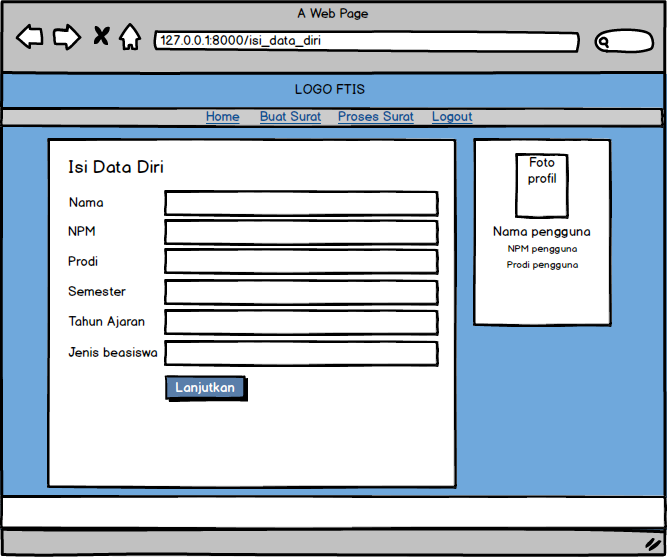
\includegraphics[scale=0.4]{F:/Skripsi/Dokumentasi_Skripsi/Gambar/Mock_Up/Mahasiswa/pengisian_data.png}
		\caption{Contoh halaman pengisian data surat}
		\label{fig:contoh_halaman_pengisian_data_surat}
	\end{figure}
	
	Apabila semua data telah diisikan pada halaman pengisian data, mahasiswa akan diarahkan ke halaman \textit{preview} untuk melihat apakah data isiannya sudah benar atau belum. Apabila data isian sudah benar mahasiswa dapat menekan tombol "Buat Surat", namun apabila ada data yang hendak diperbaiki mahasiswa dapat menekan tombol kembali. Gambar \hyperlink{contoh_halaman_preview_isi_data}{4.11} menunjukkan halaman \textit{preview} isi data surat.
	\begin{figure}[H]
	\centering
		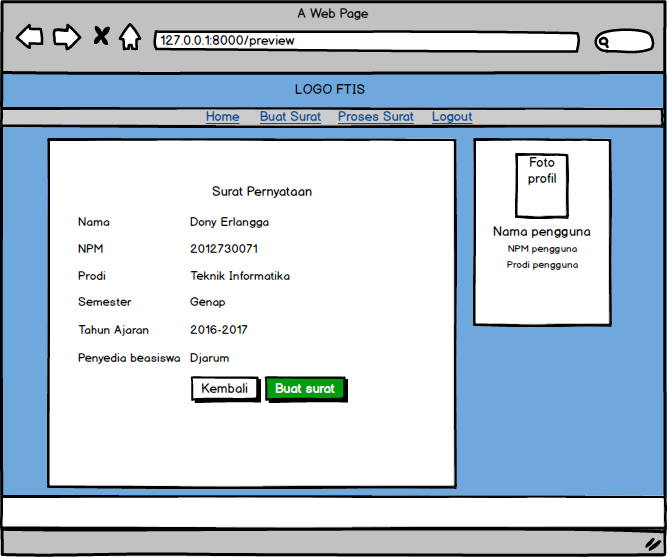
\includegraphics[scale=0.4]{F:/Skripsi/Dokumentasi_Skripsi/Gambar/Mock_Up/Mahasiswa/preview_isian_data.png}
		\caption{Contoh halaman preview isi data}
		\label{fig:contoh_halaman_preview_isi_data}
	\end{figure}
\end{enumerate}

\subsection{Perancangan Antar Muka Untuk Pejabat}
\label{sec:perancangan_antar_muka_pejabat}
Berdasarkan struktur modul, pejabat dapat menjalankan 3 fungsi yaitu melihat pesanan surat, menambahkan persetujuan dan catatan dan mengubah status penandatanganan surat yang sudah dibuat yang akan dijelaskan sebagai berikut :
\begin{enumerate}
	\item Melihat pesanan surat\\
	Surat-surat yang pernah dibuat oleh mahasiswa akan ditampilkan pada halaman \textit{home pejabat}. Gambar \hyperlink{home_pejabat_saat_ada_pesanan_surat}{4.12} menunjukkan halaman \textit{home pejabat} yang menampilkan surat yang sudah pernah dibuat.
	\begin{figure}[H]
	\centering
		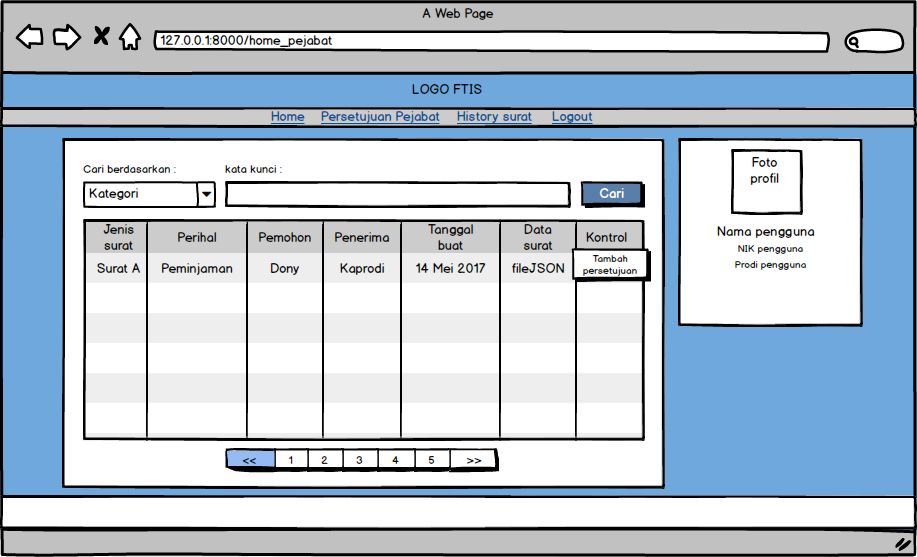
\includegraphics[scale=0.4]{F:/Skripsi/Dokumentasi_Skripsi/Gambar/Mock_Up/Pejabat/home_pejabat.png}
		\caption{Home pejabat saat ada pesanan surat}
		\label{fig:home_pejabat_saat_ada_pesanan_surat}
	\end{figure}
	
	Apabila belum ada pesanan surat, maka tampilan untuk halaman \textit{home pejabat} akan menampilkan seperti pada gambar \hyperlink{home_pejabat_saat_belum_ada_pesanan_surat}{4.13} berikut. 
	\begin{figure}[H]
	\centering
		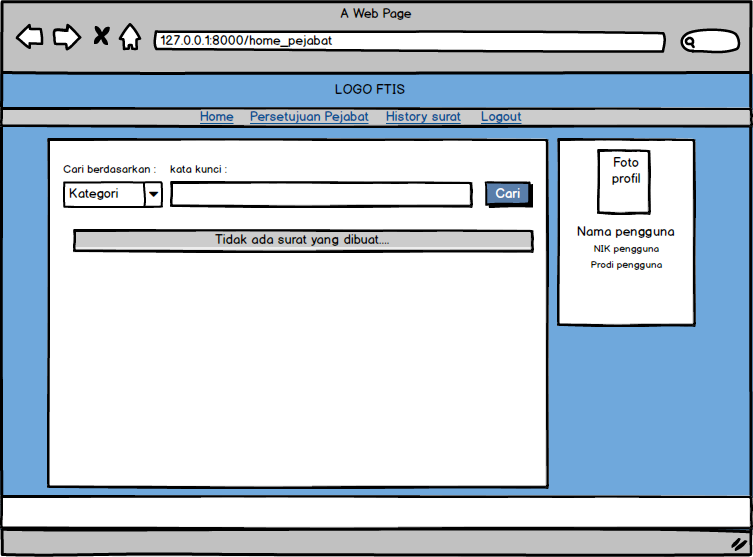
\includegraphics[scale=0.4]{F:/Skripsi/Dokumentasi_Skripsi/Gambar/Mock_Up/Pejabat/home_pejabat_kosong.png}
		\caption{Home pejabat saat belum ada pesanan surat}
		\label{fig:home_pejabat_saat_belum_ada_pesanan_surat}
	\end{figure}
	
	\item Menambahkan persetujuan dan catatan\\
	Untuk menambahkan persetujuan dan catatan pejabat perlu masuk ke halaman \textit{home pejabat} dengan menekan tombol "Home" pada \textit{navigation bar}. Pada pojok kanan tabel terdapat tombol "Tambah Catatan" yang apabila di tekan akan mengarahkan pejabat ke halaman pengisian persetujuan dan catatan. Gambar \hyperlink{halaman_pengisian_persetujuan_dan_catatan}{4.14} menunjukkan halaman \textit{home pejabat} yang menampilkan surat yang sudah pernah dibuat.
	\begin{figure}[H]
	\centering
		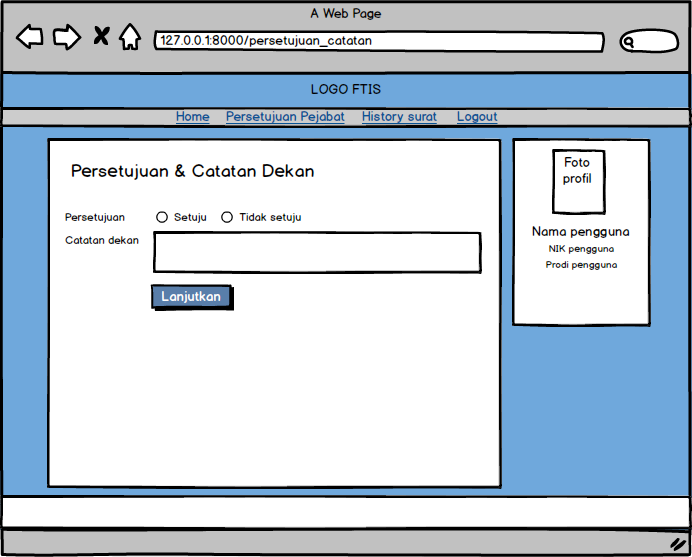
\includegraphics[scale=0.4]{F:/Skripsi/Dokumentasi_Skripsi/Gambar/Mock_Up/Pejabat/persetujuan_catatan.png}
		\caption{Halaman pengisian persetujuan dan catatan}
		\label{fig:halaman_pengisian_persetujuan_dan_catatan}
	\end{figure}
	
	Apabila persetujuan telah diisikan pada halaman pengisian persetujuan dan catatan, pejabat akan diarahkan ke halaman selanjutnya untuk melihat apakah data isiannya sudah benar atau belum. Apabila data isian sudah benar pejabat dapat menekan tombol "Kirim", namun apabila ada data yang hendak diperbaiki pejabat dapat menekan tombol kembali. Gambar \hyperlink{halaman_preview_persetujuan_dan_catatan}{4.15} menunjukkan halaman \textit{preview} persetujuan dan catatan.
	\begin{figure}[H]
	\centering
		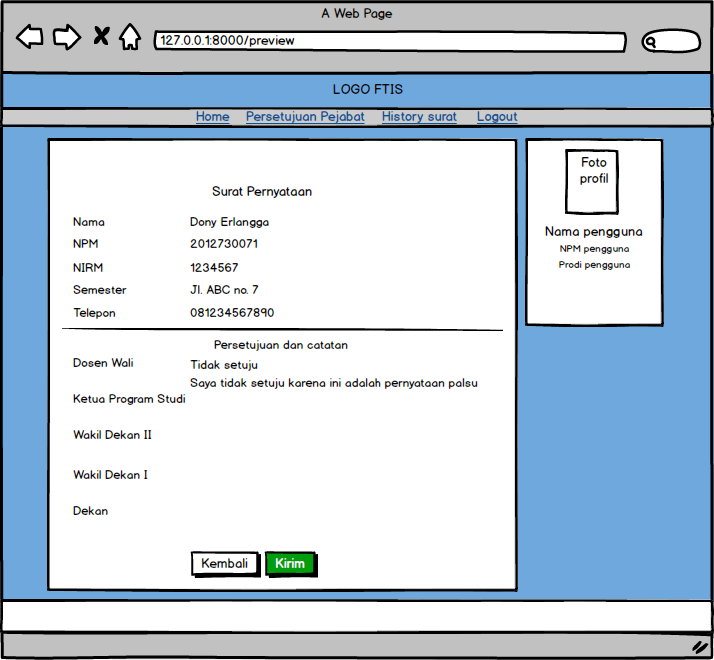
\includegraphics[scale=0.4]{F:/Skripsi/Dokumentasi_Skripsi/Gambar/Mock_Up/Pejabat/preview_persetujuan_catatan.png}
		\caption{Contoh halaman preview persetujuan dan catatan}
		\label{fig:halaman_preview_persetujuan_dan_catatan}
	\end{figure}
	
	\item Mengubah status penandatanganan surat \\
	Untuk mengubah status penandatanganan surat, petugas TU harus masuk ke halaman \textit{history} surat dan menekan tombol "Belum" pada kolom penandatanganan pada tabel \textit{history} surat. Gambar \hyperlink{halaman_history_pejabat}{4.16} merupakan halaman \textit{history} surat pada pejabat.
	\begin{figure}[H]
	\centering
		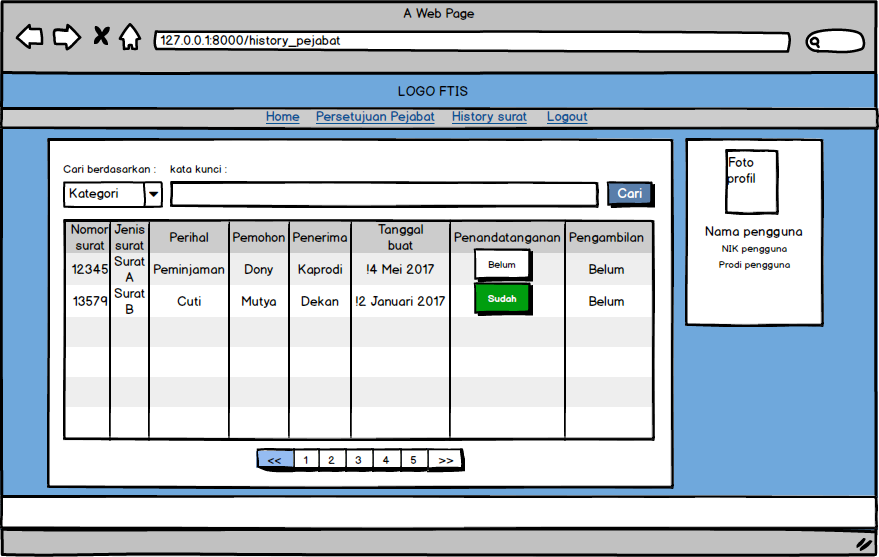
\includegraphics[scale=0.4]{F:/Skripsi/Dokumentasi_Skripsi/Gambar/Mock_Up/pejabat/history_pejabat.png}
		\caption{Halaman \textit{history} pejabat}
		\label{fig:halaman_history_pejabat}
	\end{figure}

	\item Cek persetujuan pejabat
	Pejabat dapat memantau proses persetujuan surat yang dipesan oleh mahasiswa bimbingannya pada halaman persetujuan pejabat yang ditampilkan pada gambar \hyperlink{halaman_persetujuan_pejabat}{4.17}.
	\begin{figure}[H]
	\centering
		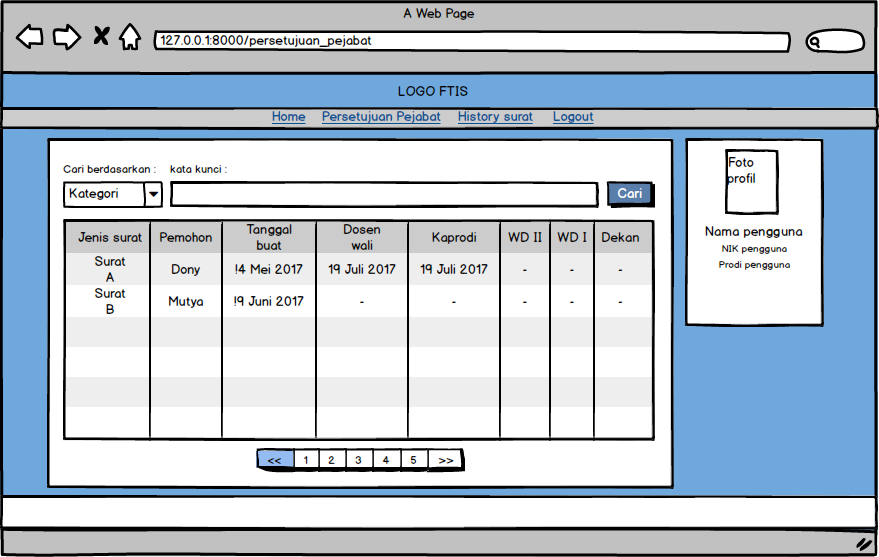
\includegraphics[scale=0.4]{F:/Skripsi/Dokumentasi_Skripsi/Gambar/Mock_Up/Pejabat/persetujuan_pejabat.png}
		\caption{Halaman persetujuan pejabat}
		\label{fig:halaman_persetujuan_pejabat}
	\end{figure}
\end{enumerate}

\subsection{Perancangan Antar Muka Untuk Petugas TU}
\label{sec:perancangan_antar_muka_petugas_tu}
Berdasarkan struktur modul, petugas TU dapat menjalankan 4 fungsi yaitu menambahkan nomor surat dan meng-\textit{generate} surat, menambahkan list data mahasiswa dan format surat baru dan mengubah status pengambilan surat yang sudah dibuat yang akan dijelaskan sebagai berikut :
\begin{enumerate}
	\item Menambahkan nomor surat dan meng-\textit{generate} surat \\
	Untuk menambahkan nomor surat dan meng-\textit{generate} surat petugas TU harus menekan tombol "Tambah Nomor Surat" pada bagian kanan tabel pesanan surat di halaman \textit{home} petugas TU. Gambar \hyperlink{halaman_home_TU}{4.18} menunjukkan halaman \textit{home} petugas TU.
	\begin{figure}[H]
	\centering
		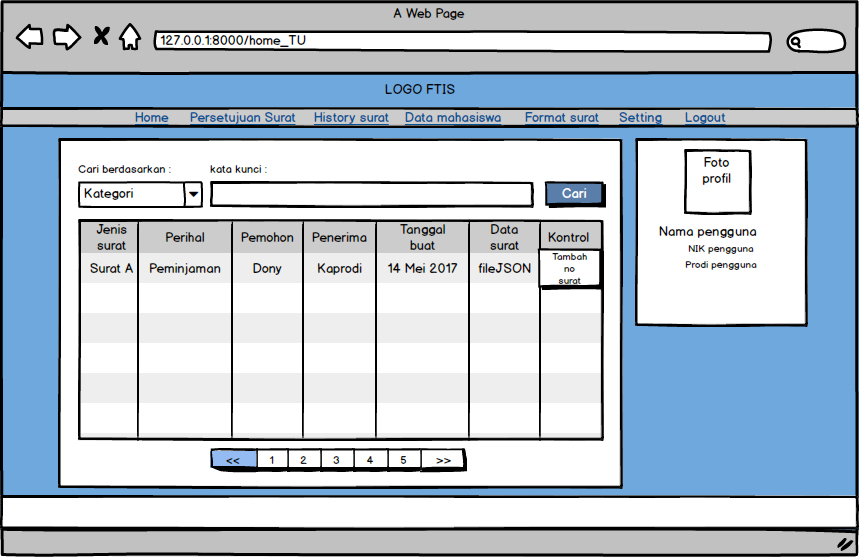
\includegraphics[scale=0.4]{F:/Skripsi/Dokumentasi_Skripsi/Gambar/Mock_Up/TU/home_TU.png}
		\caption{Halaman \textit{home} TU}
		\label{fig:halaman_home_TU}
	\end{figure}
	
	Setelah menekan tombol "Tambah Nomor Surat", petugas TU akan diarahkan menuju halaman pengisisan nomor surat. Apabila nomor surat sudah diisi, petugas TU dapat menekan tombol "Buat Surat (PDF)". Gambar \hyperlink{isi_nomor_surat}{4.19} menunjukkan halaman pengisisan nomor surat.
	\begin{figure}[H]
	\centering
		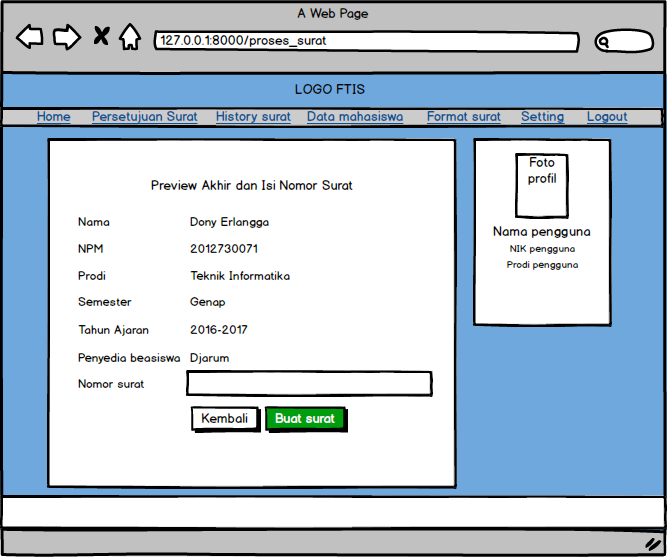
\includegraphics[scale=0.4]{F:/Skripsi/Dokumentasi_Skripsi/Gambar/Mock_Up/TU/noSurat.png}
		\caption{Halaman menambahkan nomor surat}
		\label{fig:isi_nomor_surat}
	\end{figure}
	
	\item Menambahkan format surat baru\\
	Untuk menambahkan format surat baru petugas TU harus masuk terlebih dahulu ke halaman \textit{format surat} dengan menekan tombol "Format Surat" pada \textit{navigation bar} yang ditunjukkan pada gambar \hyperlink{halaman_format_surat}{4.20}.
	\begin{figure}[H]
	\centering
		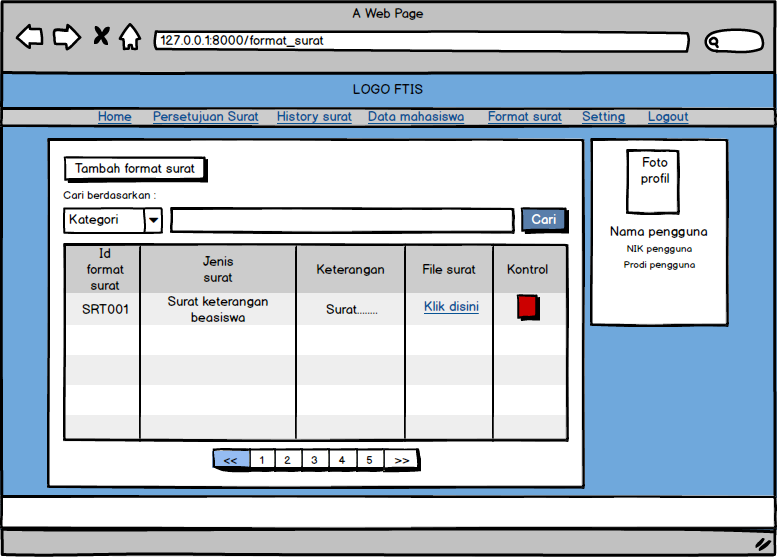
\includegraphics[scale=0.4]{F:/Skripsi/Dokumentasi_Skripsi/Gambar/Mock_Up/TU/format_surat.png}
		\caption{Halaman format surat}
		\label{fig:halaman_format_surat}
	\end{figure}
	
	Pada halaman \textit{format surat} terdapat tombol "Tambah format surat" yang apabila ditekan maka petugas TU akan diarahkan ke halaman untuk mengisi id dari format surat, nama surat, keterangan dan meng-\textit{upload} format surat baru yang ditunjukkan pada gambar \hyperlink{halaman_tambah_format_surat}{4.21}.
	\begin{figure}[H]
	\centering
		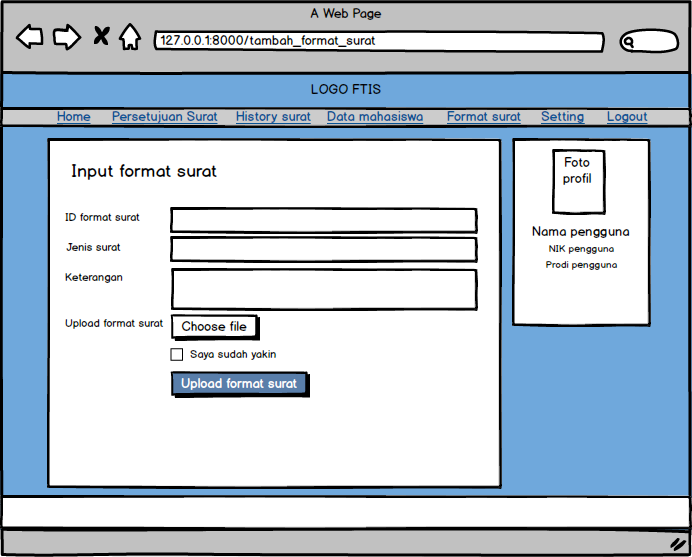
\includegraphics[scale=0.4]{F:/Skripsi/Dokumentasi_Skripsi/Gambar/Mock_Up/TU/tambah_format_surat.png}
		\caption{Halaman tambah format surat}
		\label{fig:halaman_tambah_format_surat}
	\end{figure}
	
	\item Mengubah status pengambilan surat\\
	Untuk mengubah status pengambilan surat, petugas TU harus masuk ke halaman \textit{history} surat dan menekan tombol "Belum" pada kolom pengambilan pada tabel \textit{history} surat. Gambar \hyperlink{halaman_history_TU}{4.22} merupakan halaman \textit{history} surat pada petugas TU.
	\begin{figure}[H]
	\centering
		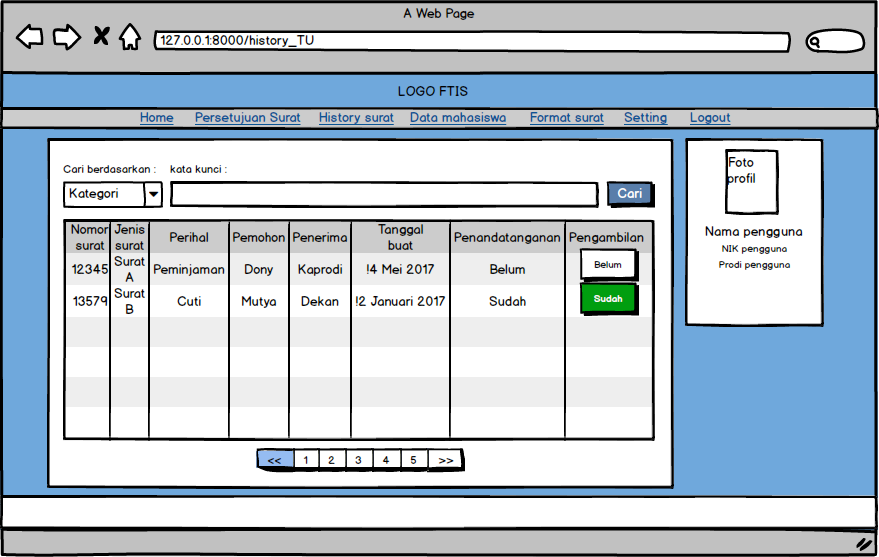
\includegraphics[scale=0.4]{F:/Skripsi/Dokumentasi_Skripsi/Gambar/Mock_Up/TU/history_TU.png}
		\caption{Halaman \textit{history} TU}
		\label{fig:halaman_history_TU}
	\end{figure}
	
	\item Mengubah semester dan tahun akademik terkini \\
	Untuk mengubah semester dan tahun akademik terkini petugas TU harus masuk terlebih dahulu ke halaman \textit{setting} dengan menekan tombol "Setting" pada \textit{navigation bar}. Gambar \hyperlink{setting}{4.23} merupakan halaman pengaturan semester dan tahun akademik.
	\begin{figure}[H]
	\centering
		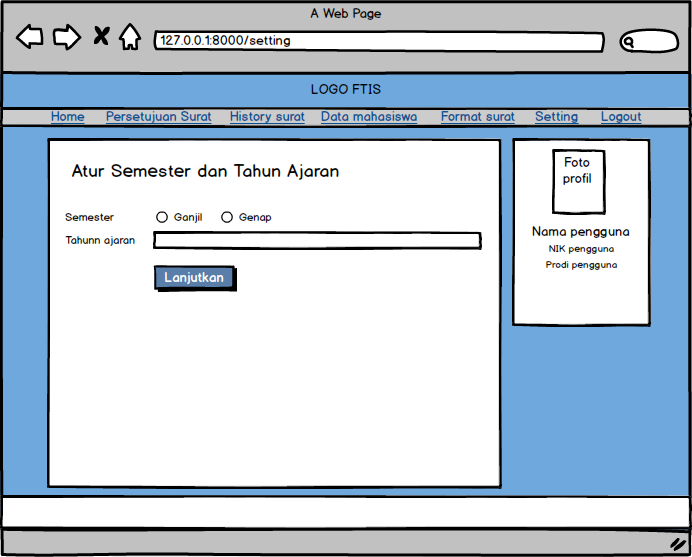
\includegraphics[scale=0.4]{F:/Skripsi/Dokumentasi_Skripsi/Gambar/Mock_Up/TU/setting.png}
		\caption{Halaman \textit{setting} semester dan tahun ajaran}
		\label{fig:setting}
	\end{figure}
	
	\item Cek persetujuan surat
	Petugas TU dapat memantau proses persetujuan surat yang dipesan oleh seluruh mahasiswa pada halaman persetujuan surat yang ditampilkan pada gambar \hyperlink{halaman_persetujuan_surat}{4.24}.
	\begin{figure}[H]
	\centering
		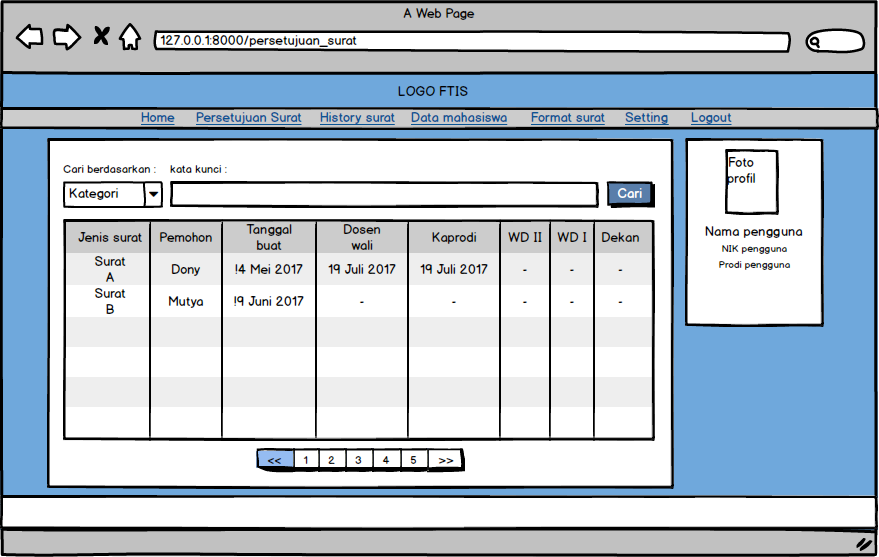
\includegraphics[scale=0.4]{F:/Skripsi/Dokumentasi_Skripsi/Gambar/Mock_Up/TU/persetujuan_surat.png}
		\caption{Halaman persetujuan surat}
		\label{fig:halaman_persetujuan_surat}
	\end{figure}
\end{enumerate}
